\begin{center}
     \huge BÁO CÁO THÍ NGHIỆM VI SINH VẬT \\ \vspace{10pt}
  \huge Bài 2: Phân lập VSV hiếu khí và VSV yếm khí.
\end{center}

\section{Mục đích thí nghiệm}

\begin{itemize}
    \item Thành thạo kỹ năng phân lập vi sinh vật trên canh trường thuần khiết bằng phương pháp gieo cấy trên môi trường đặc.
    \item Thành thạo về kỹ thuật gieo cấy vi sinh vật (gieo cấy vi sinh vật bằng pipet và que chang).
    \item Biết cách phân lập vi sinh vật hiếu khí và vi sinh vật yếm khí.
\end{itemize}

\section{Vật liệu và phương pháp thí nghiệm}

\subsection{Vật liệu thí nghiệm}

\begin{itemize}
    \item Pipette 1000, 100 và hộp đầu côn.
    \item Ống eff, bình tam giác, hộp petri nhựa, falcon 50 mL, que chang.
    \item Cồn sát khuẩn, bông thấm, đèn cồn, ống nghiệm, nồi hấp thanh trùng, vortex.
    \item Hóa chất: môi trường MRS, Agar 2\% và môi trường Shapek + CaC$O_3$.
    \item Mẫu: kim chi, bánh men.
\end{itemize}

\subsection{Phương pháp thí nghiệm}

\begin{itemize}
    \item Pha chế 50 mL môi trường MRS.
    \item Lấy 50 mL nước vào 2 lọ côn.
    \item Lấy 99 mL nước vào 2 bình tam giác.
    \item Pha thạch agar để tạo lớp thạch yếm khí cho phân lập VSV yếm khí.
\end{itemize}

$\rightarrow$ Mang tất cả đi thanh trùng trong nồi hấp.

\subsubsection{Phương pháp phân lập vi sinh vật hiếu khí}

\textbf{Bước 1: Chuẩn bị dụng cụ phân lập.}

Trước khi tiến hành thí nghiệm với vi sinh vật thì cần phải sát trùng tay bằng dung dịch cồn 70\%, sát trùng mặt bàn làm việc trước và sau khi làm việc. Thao tác vô trùng được thực hiện trong không gian vô trùng dưới ngọn lửa đèn cồn. Sức nóng của ngọn lửa đèn cồn sẽ tạo ra một vùng không khí nhỏ vô trùng xung quanh nó.

\textbf{Bước 2: Thao tác phân lập, cấy truyền.}

Pha loãng dịch huyền phù: Lấy 1g mẫu bánh men đã được nghiền nhỏ cho vào bình tam giác có 99 mL nước muối sinh lý, lắc đều. Lấy 100 $\mu$L dịch bánh men đang ở độ pha loãng 10$^{-2}$ cho vào ống nghiệm có 900 $\mu$L nước muối sinh lý, lắc đều bằng vortex, ta được dung dịch có độ pha loãng 10$^{-3}$. Tiếp tục làm tương tự trên để ta pha loãng dịch canh trường được các nồng độ thấp hơn: 10$^{-4}$, 10$^{-5}$ và 10$^{-6}$.

\textbf{Bước 3: Cấy truyền dịch bánh men lên môi trường thạch trong đĩa petri.}

Dùng pipet nhỏ 0.1 mL dịch huyền phù vi sinh vật lên mặt thạch trong đĩa petri. Dùng que trang đã khử trùng trải đều giọt dịch huyền phù vi sinh vật lên bề mặt thạch. Đậy nắp hộp petri, dán nhãn cho hộp petri gồm ngày thực hiện, nồng độ pha loãng của dịch huyền phù, tên môi trường. Gói hộp petri và đưa vào tủ nuôi cấy ở điều kiện thích hợp.

\subsubsection{Phương pháp phân lập vi sinh vật yếm khí}

\textbf{Bước 1: Thực hiện như bước 1 của phân lập vi sinh vật hiếu khí.}

\textbf{Bước 2: Thao tác phân lập, cấy truyền.}

Pha loãng dịch huyền phù. Dùng pipet hút 1 mL kim chi (mẫu) sau đó cho vào bình tam giác có 99 mL nước muối sinh lý, lắc đều. Lấy 100 $\mu$L dịch kim chi ở độ pha loãng 10$^{-2}$ cho vào ống nghiệm có 900 $\mu$L nước muối sinh lý, lắc đều bằng vortex, ta được dung dịch có độ pha loãng 10$^{-3}$. Tiếp tục làm tương tự ta được dịch canh trường pha loãng với các nồng độ thấp hơn: 10$^{-4}$, 10$^{-5}$ và 10$^{-6}$.

\textbf{Bước 3: Cấy truyền dịch kim chi lên môi trường thạch trong đĩa petri.}

Dùng pipet nhỏ 0.1 mL dịch huyền phù vi sinh vật lên mặt thạch trong đĩa petri. Dùng que trang đã khử trùng trải đều giọt dịch huyền phù vi sinh vật lên bề mặt thạch. Đổ lên đó một lớp thạch nước lên để tạo môi trường yếm khí. Đậy nắp hộp petri, dán nhãn cho hộp petri gồm ngày thực hiện, nồng độ pha loãng của dịch huyền phù, tên môi trường. Gói hộp petri và đưa vào tủ nuôi cấy với điều kiện thích hợp.

\subsection{Kết quả thí nghiệm}

\subsubsection{VSV hiếu khí trong bánh men}

\begin{figure}[h]
      \centering
      \subfloat{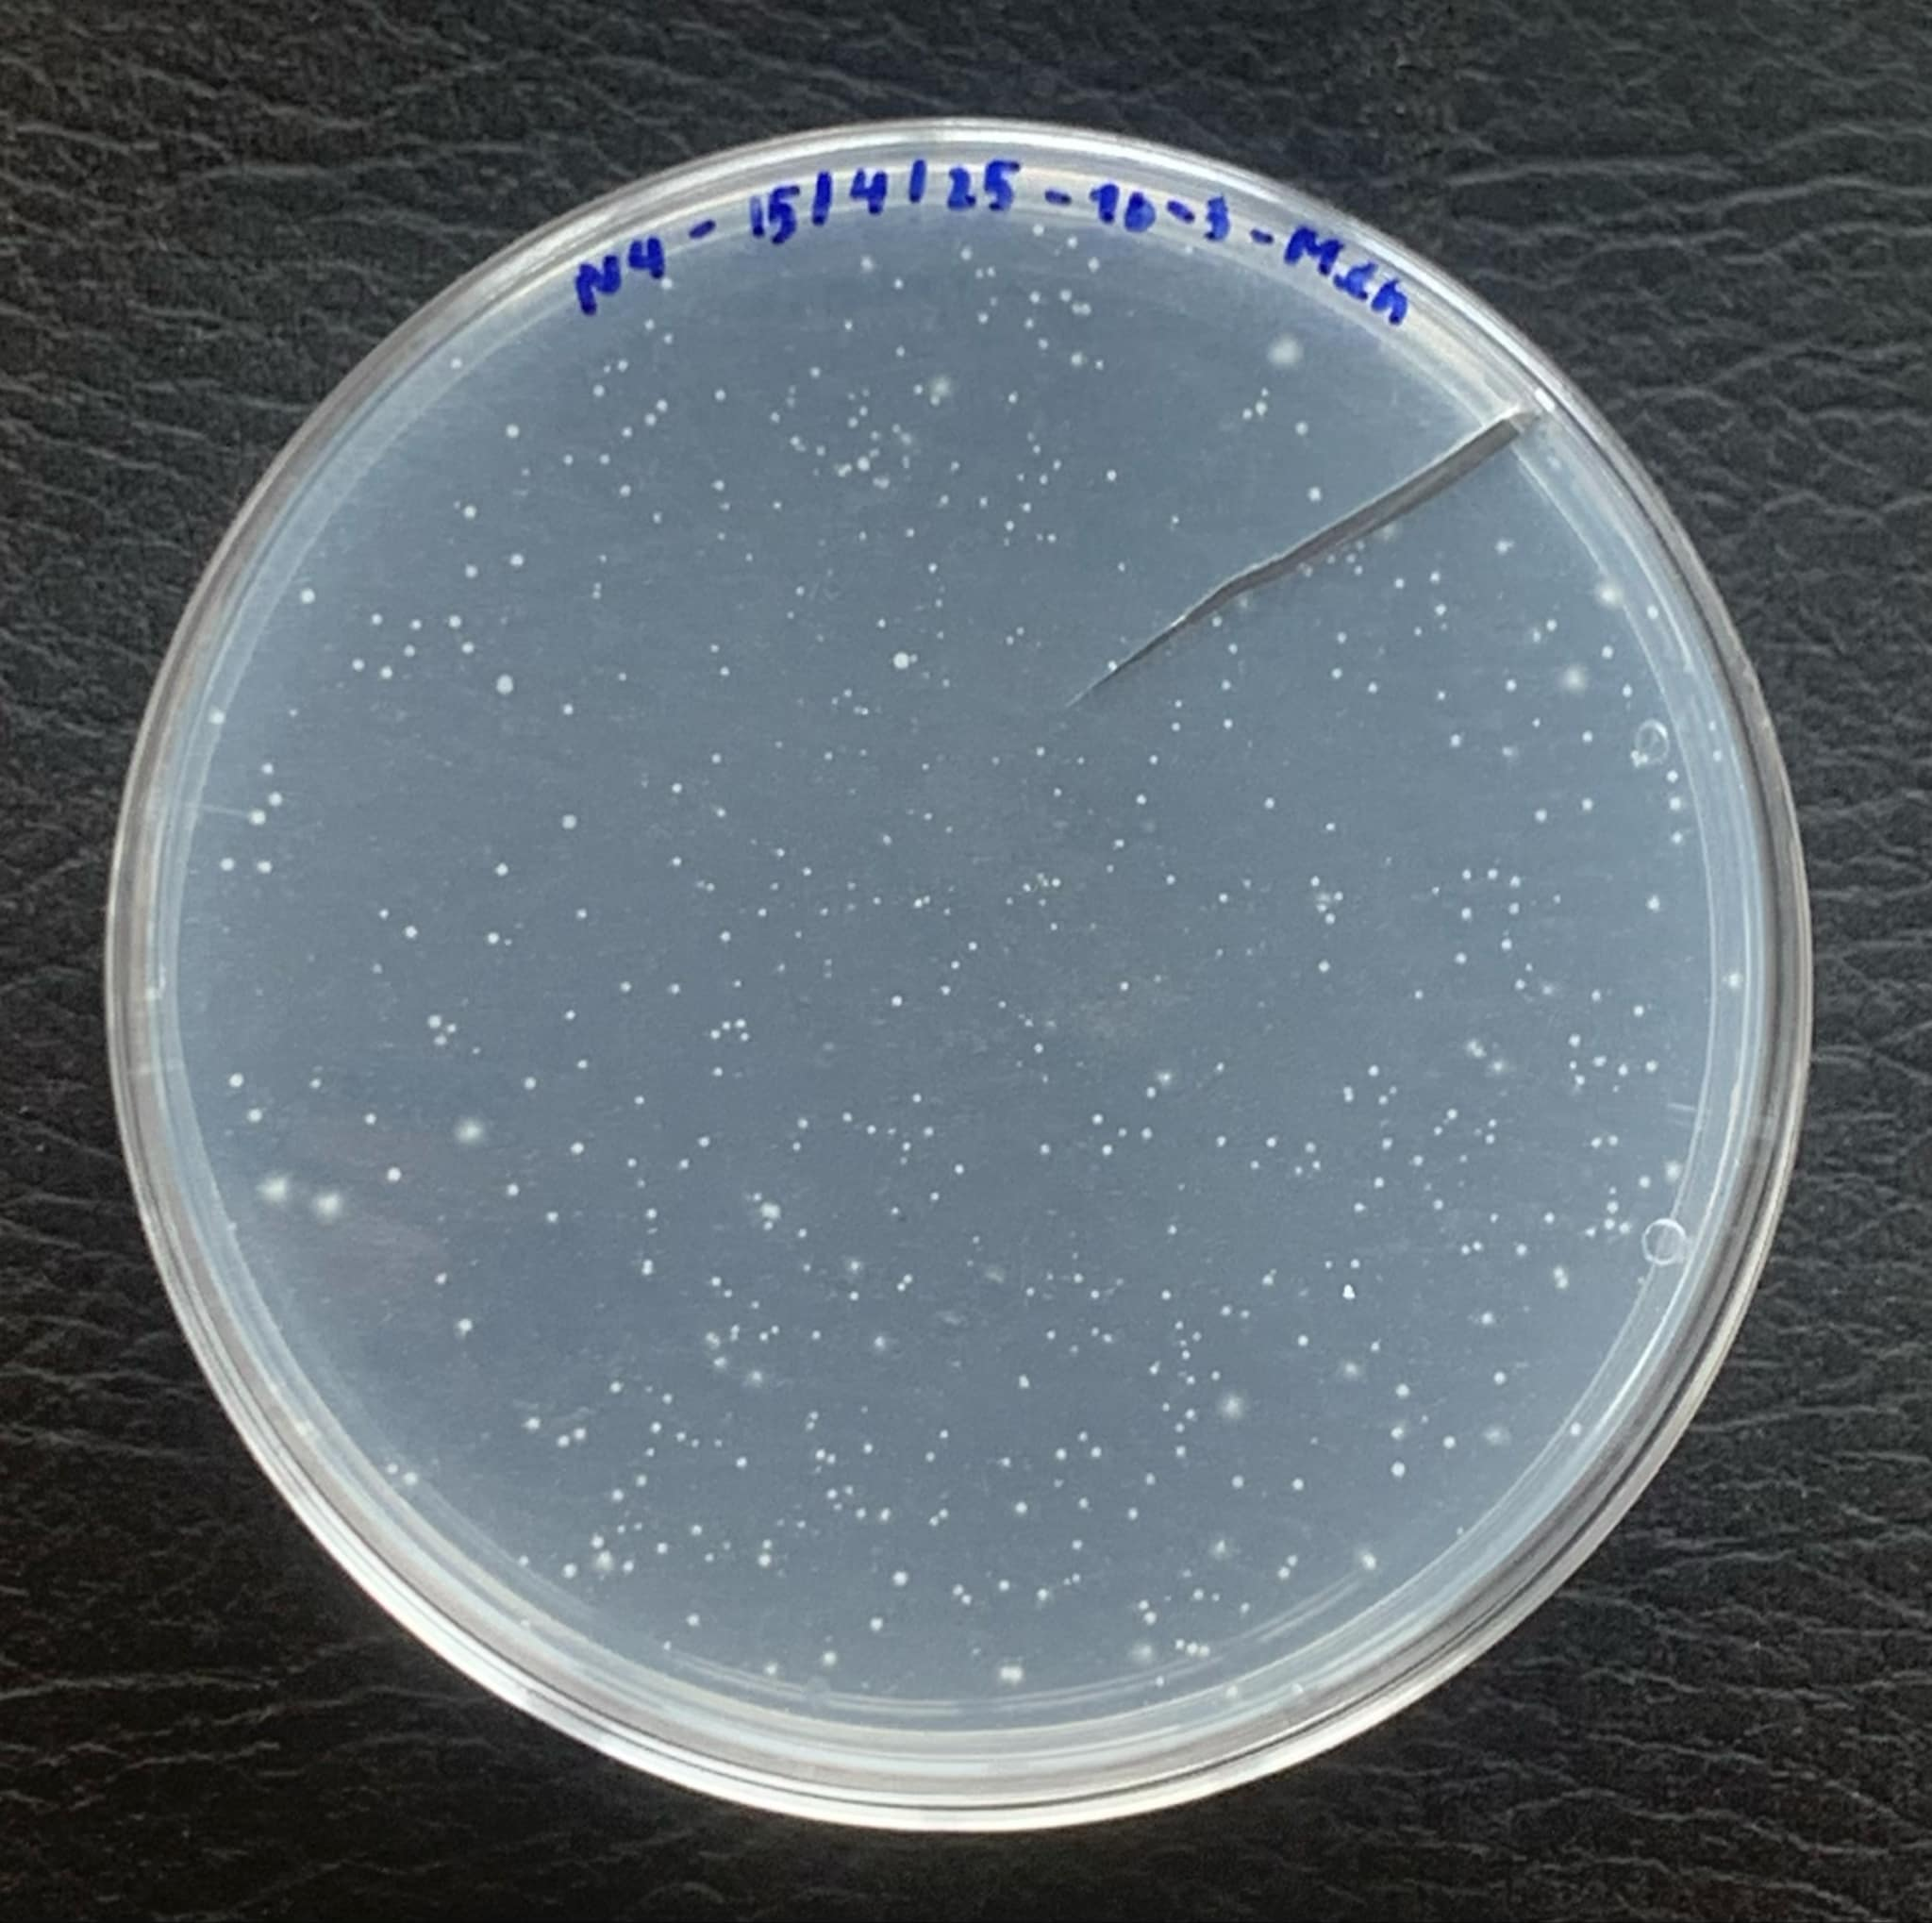
\includegraphics[width=.3\textwidth]{2-exp-2-figures/banh-men-10-^-3.jpg}}
      \qquad
      \subfloat{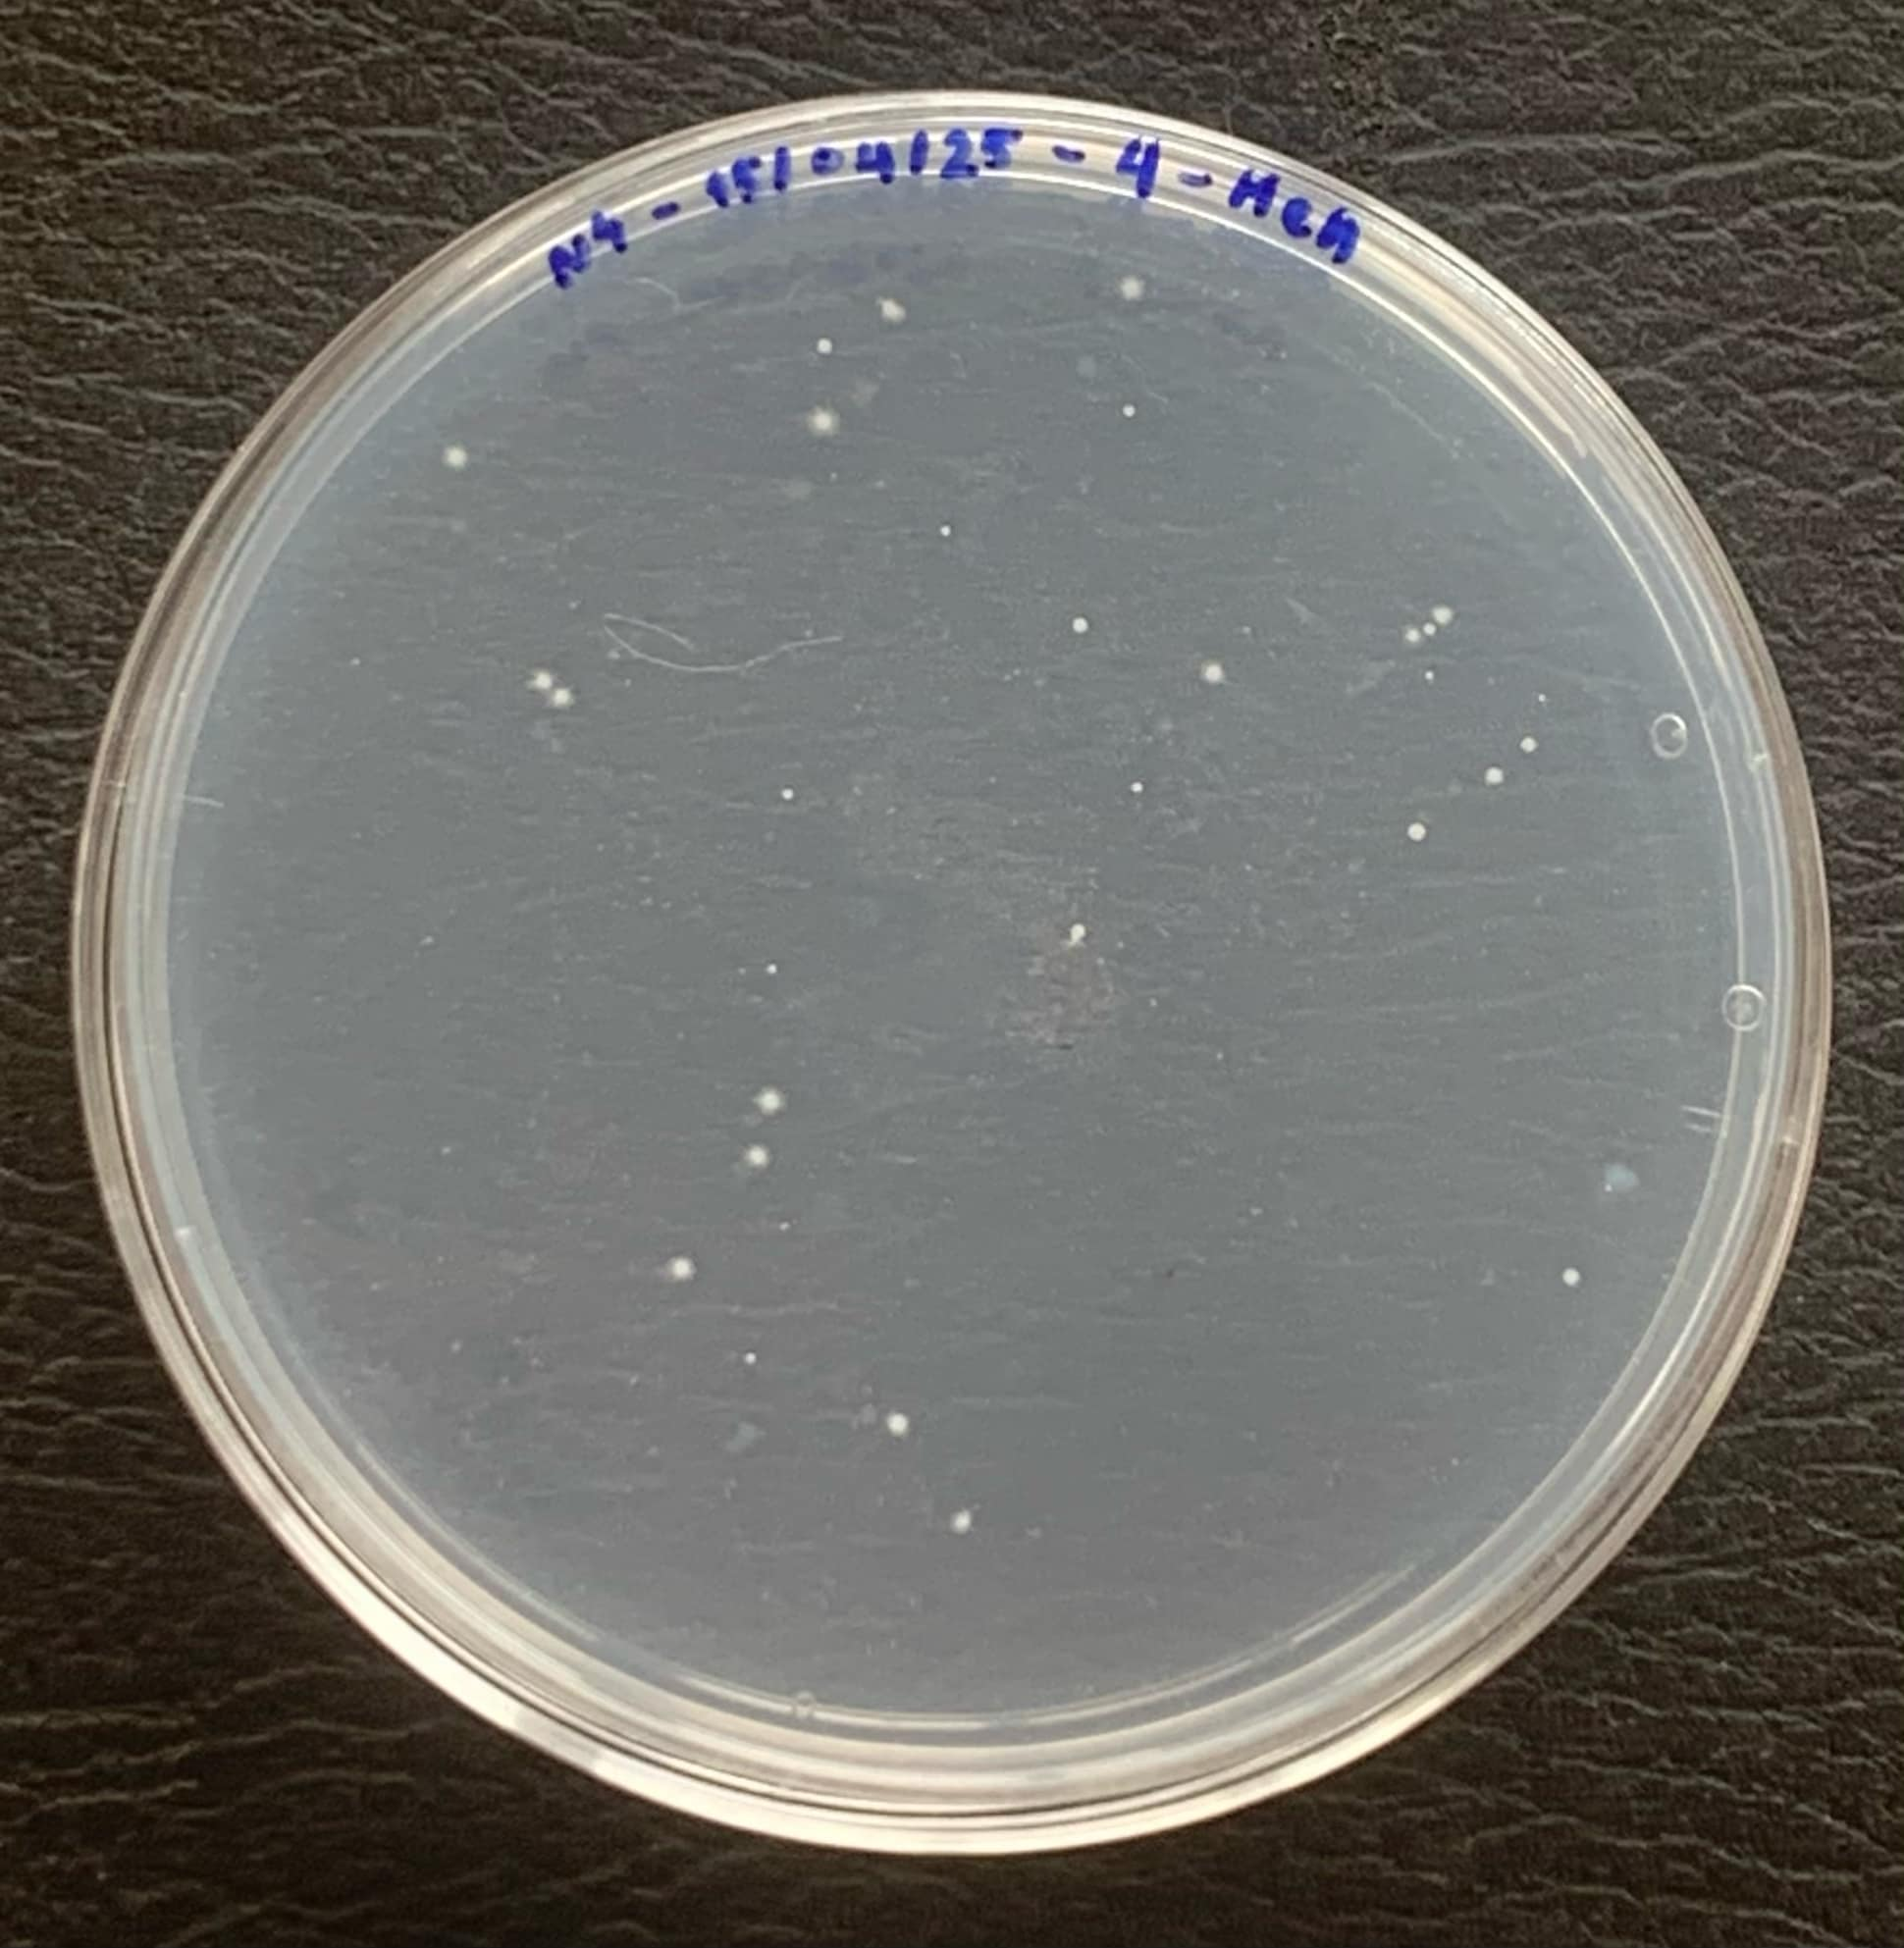
\includegraphics[width=.3\textwidth]{2-exp-2-figures/banh-men-10-^-4.jpg}}
      \qquad
      \subfloat{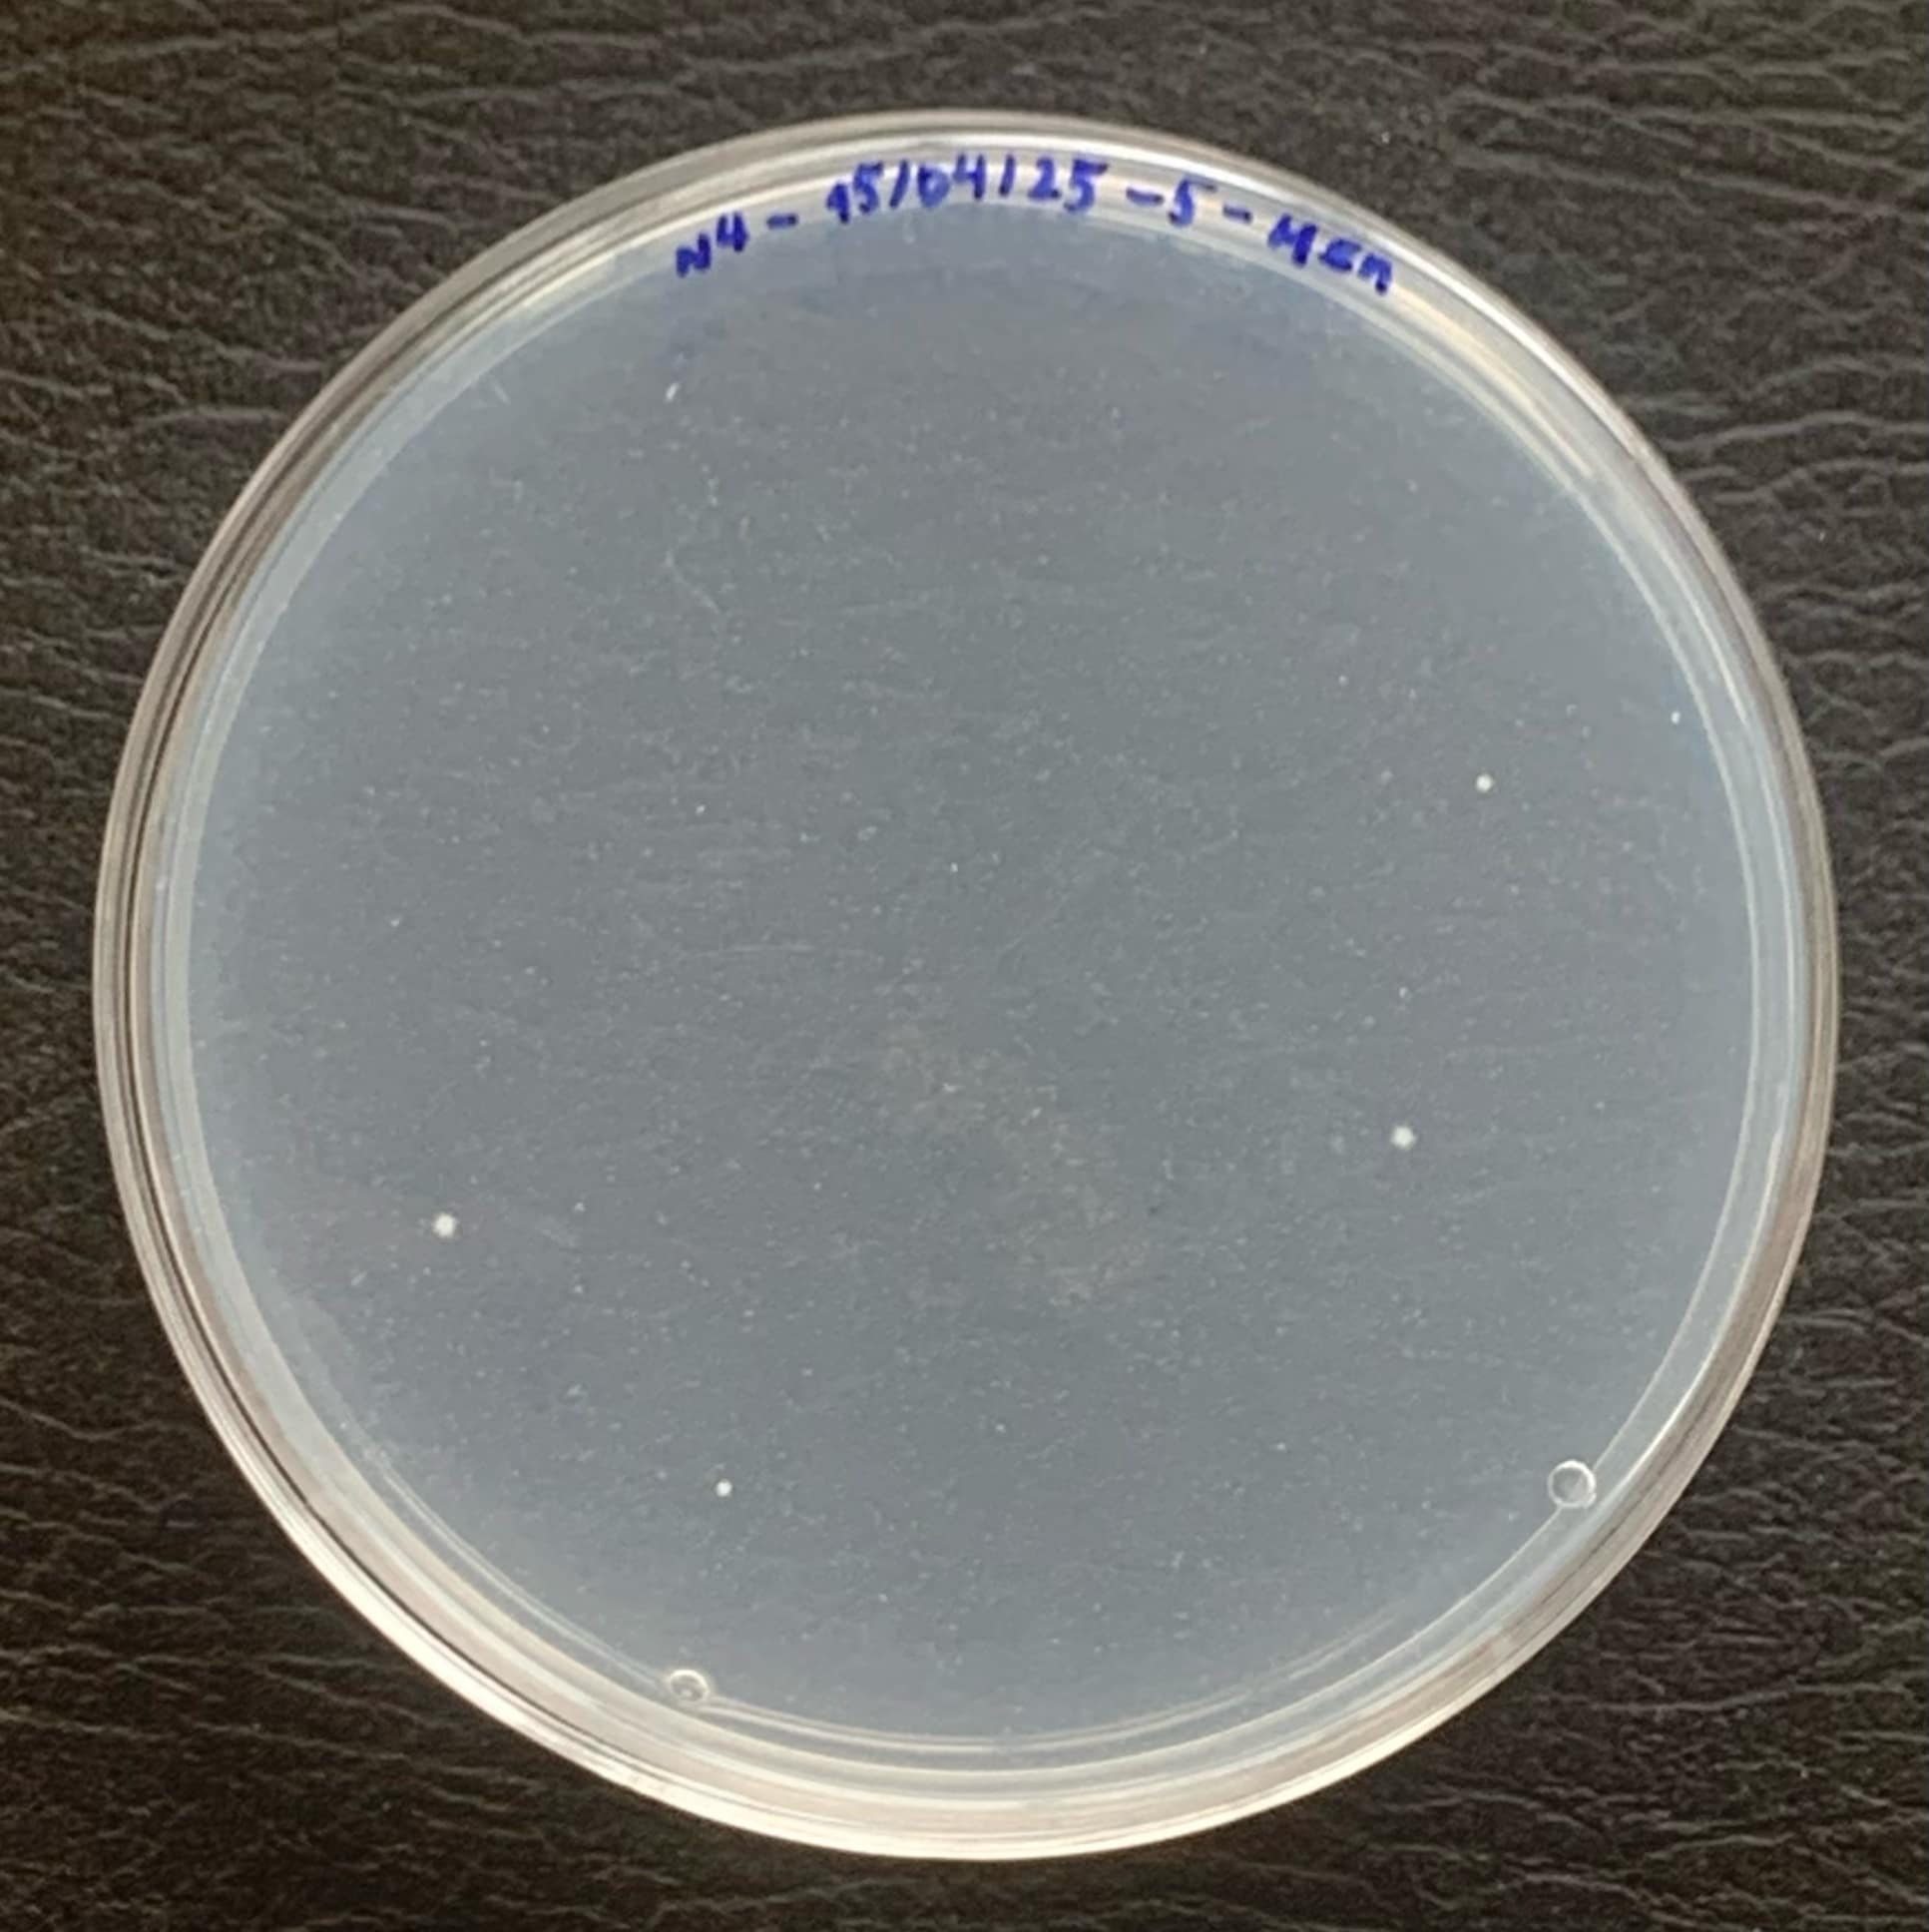
\includegraphics[width=.3\textwidth]{2-exp-2-figures/banh-men-10-^-5.jpg}}
  \caption{Mẫu bánh men với độ pha loãng lần lượt là 10$^{-3}$, 10$^{-4}$ và 10$^{-5}$.}
\end{figure}

Sau 2 ngày nuôi cấy, với độ pha loãng 10$^{-3}$ ta có thể quan sát được khá nhiều khuẩn lạc riêng biệt màu trắng, tròn xuất hiện trên bề mặt thạch, dùng que cấy lấy một ít vi sinh vật ở khuẩn lạc riêng biệt cấy chuyền lên ống thạch. Mỗi khuẩn lạc cấy lên một ống. Sau đó nuôi ở nhiệt độ thích hợp ta sẽ thu được canh trường thuần khiết. Ở độ pha loãng 10$^{-4}$ và 10$^{-5}$, đĩa petri xuất hiện tương đối ít khuẩn lạc. 

\subsubsection{VSV yếm khí trong kim chi}

\begin{figure}[h]
      \centering
      \subfloat{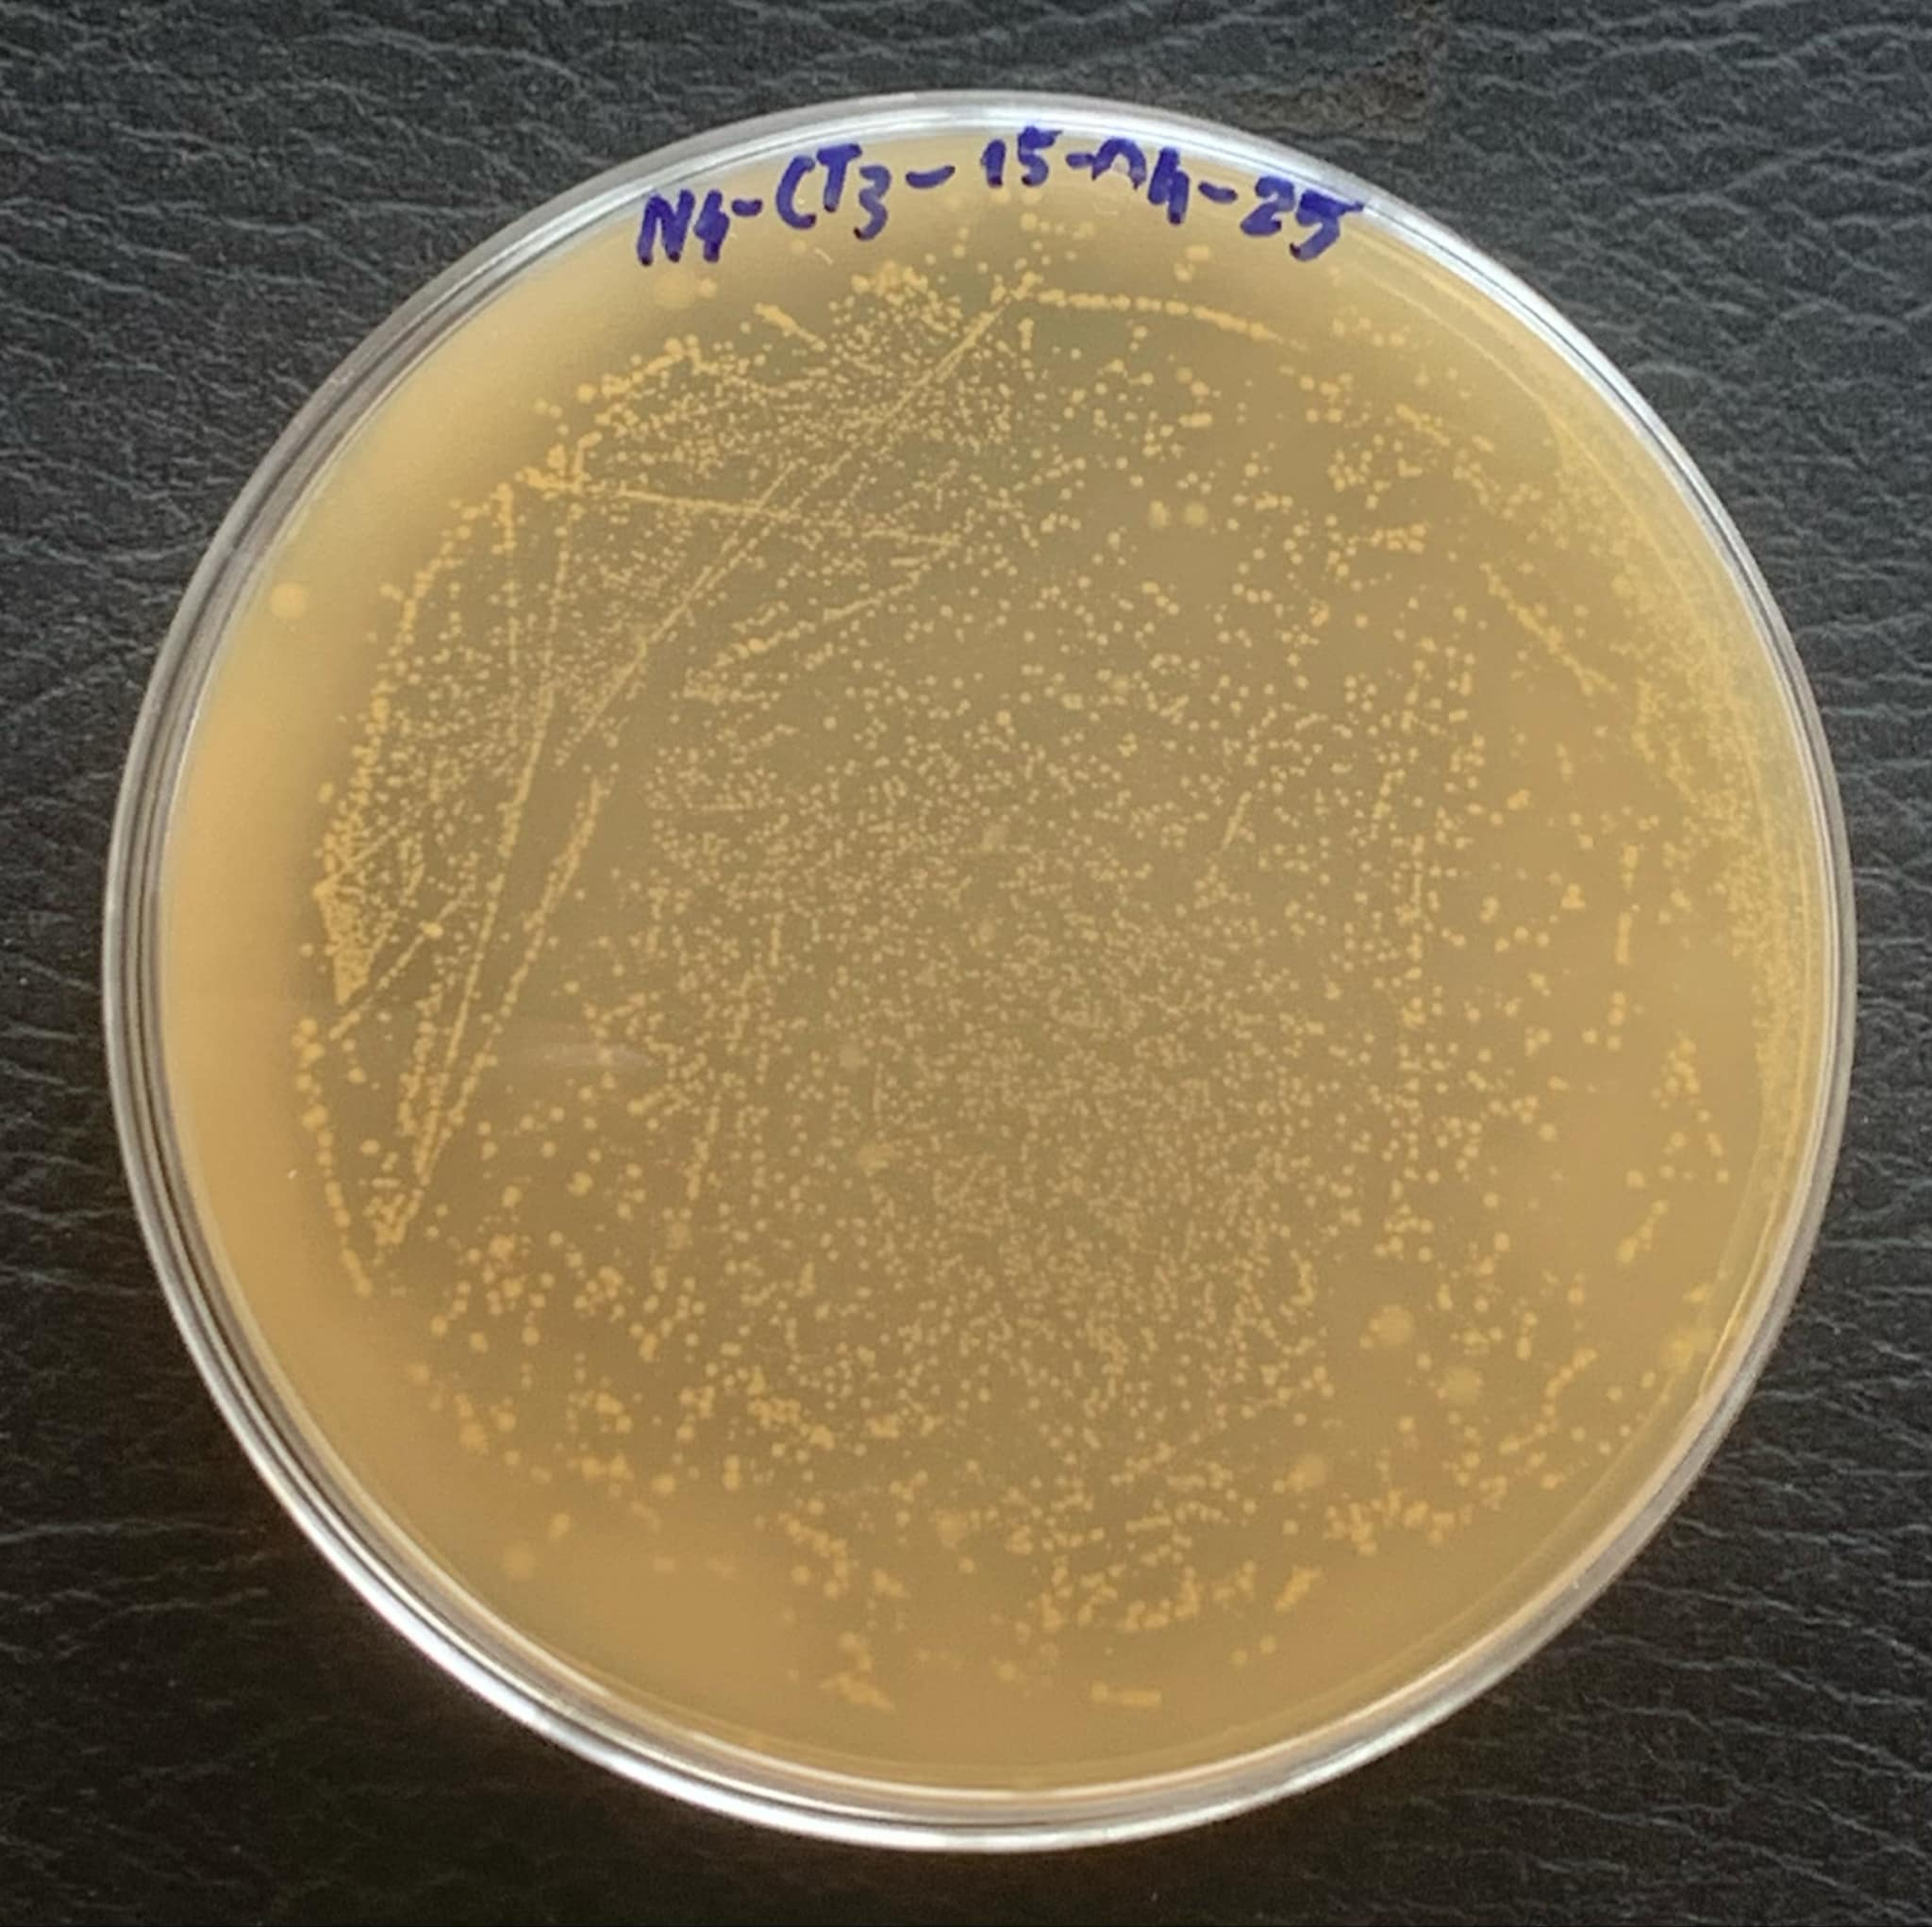
\includegraphics[width=.3\textwidth]{2-exp-2-figures/kim-chi-10-^-3.jpg}}
      \qquad
      \subfloat{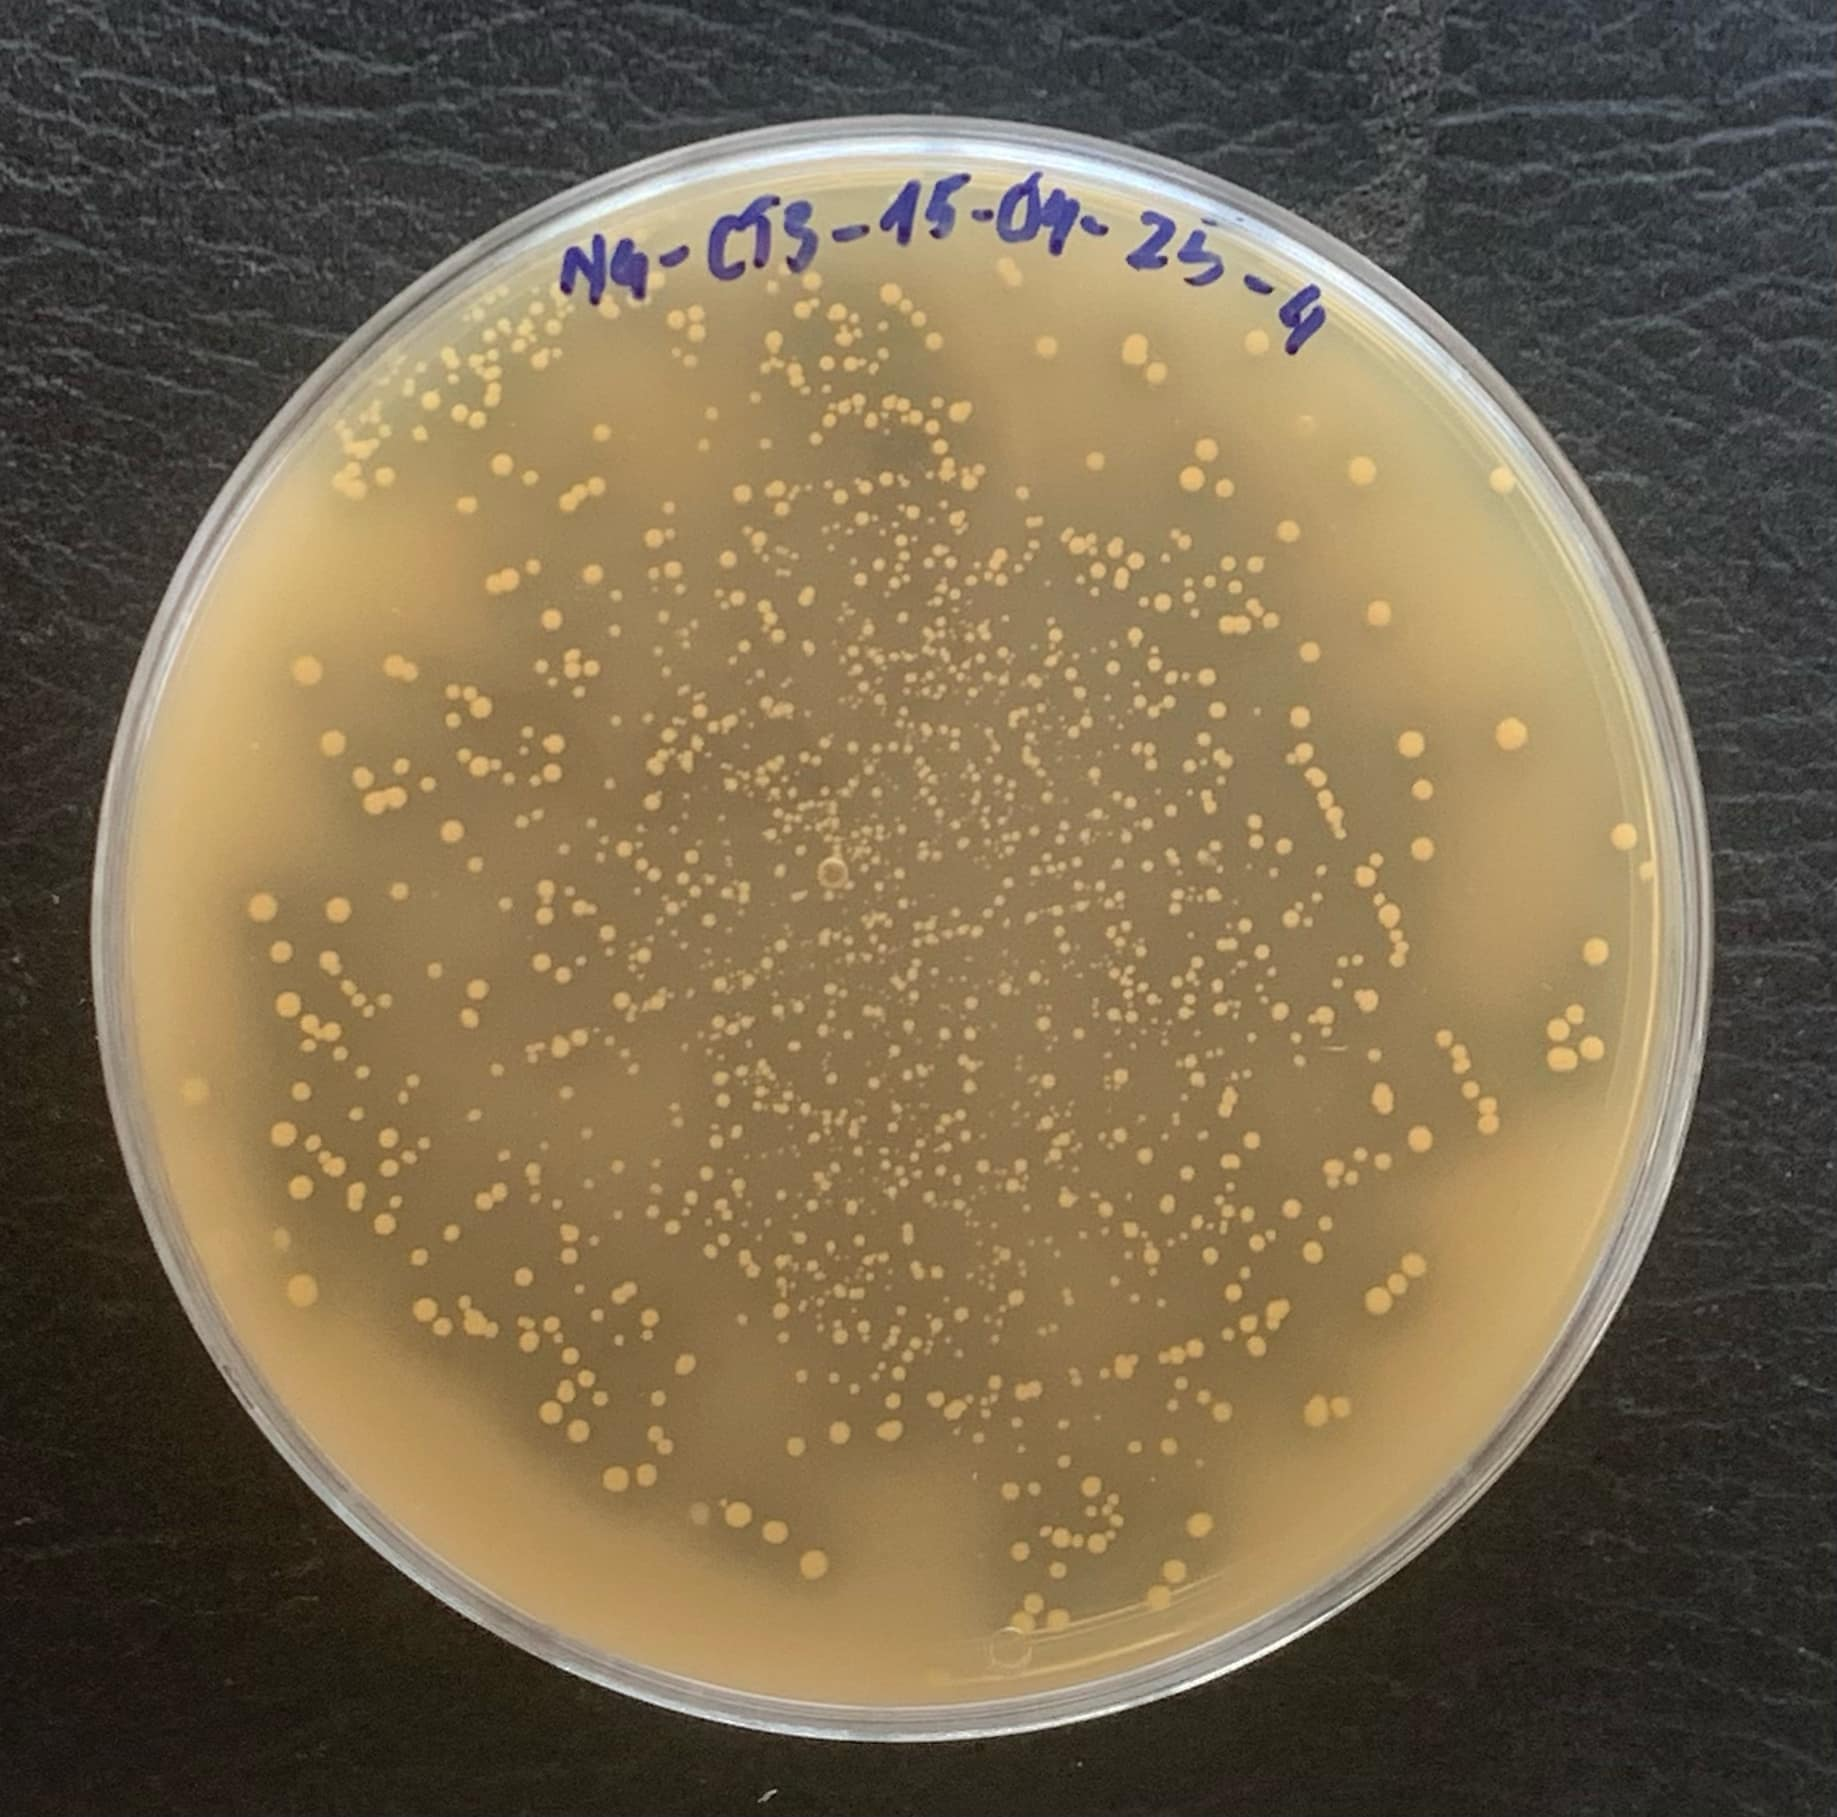
\includegraphics[width=.3\textwidth]{2-exp-2-figures/kim-chi-10-^-4.jpg}}
      \qquad
      \subfloat{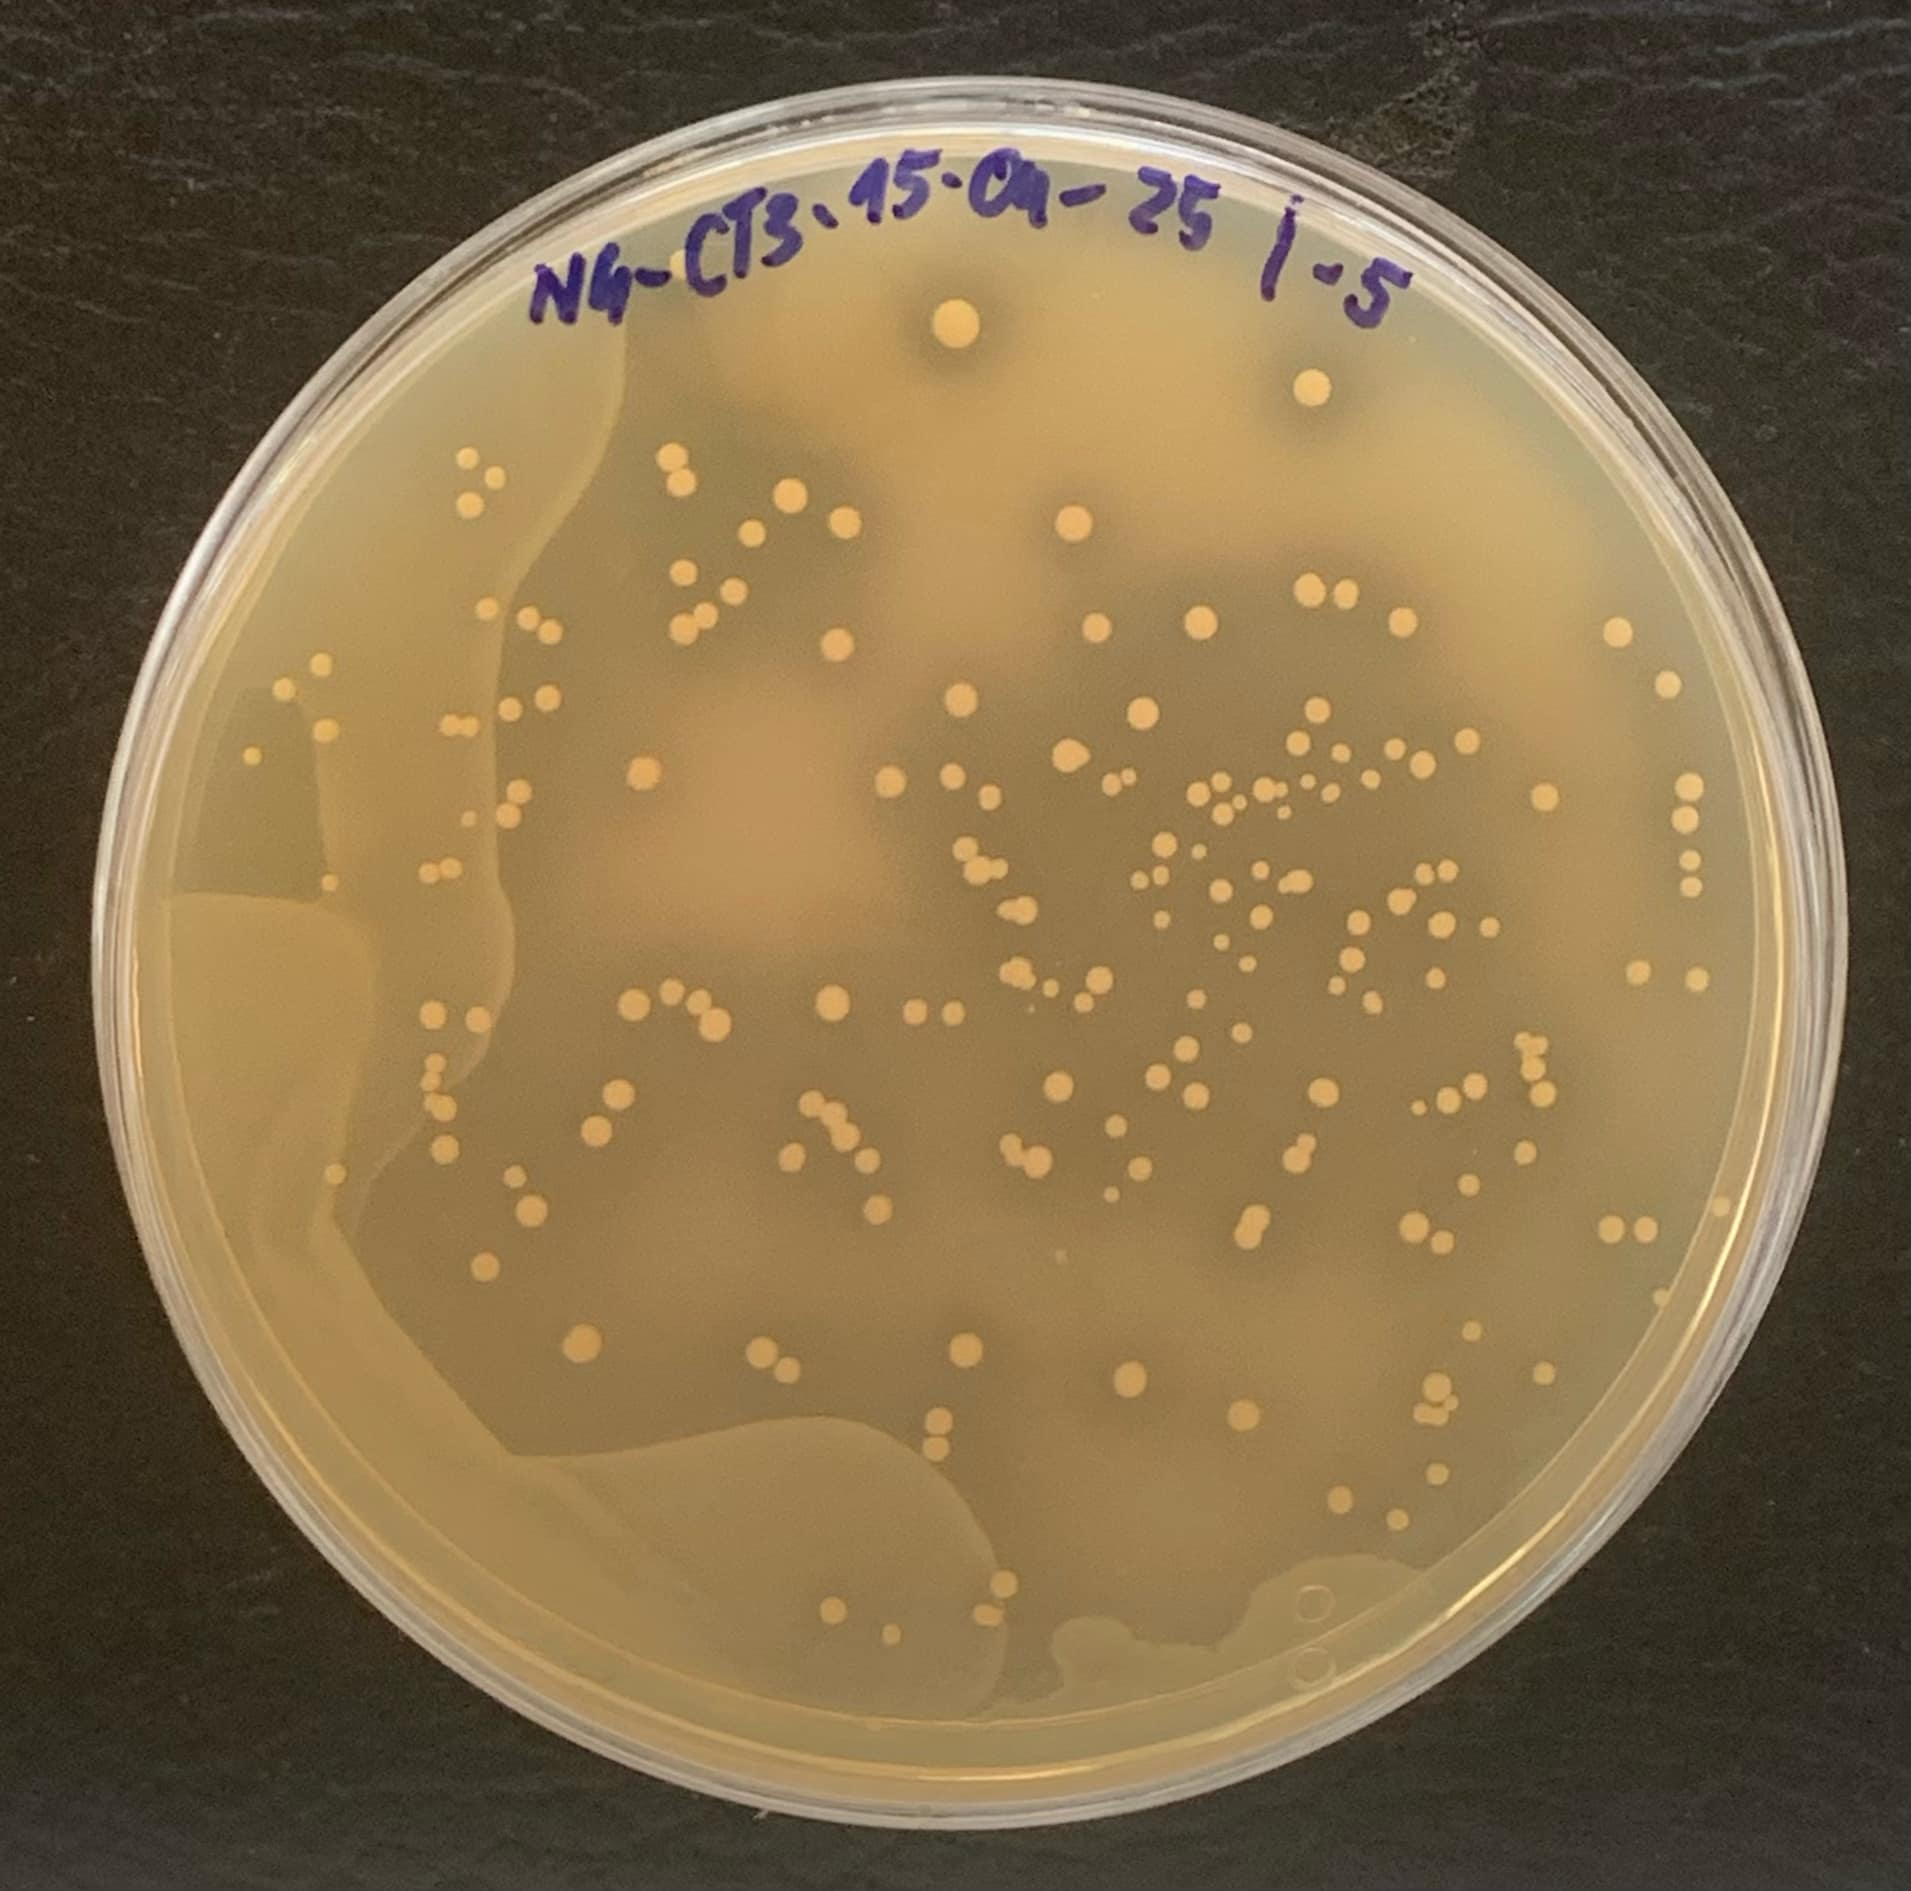
\includegraphics[width=.3\textwidth]{2-exp-2-figures/kim-chi-10-^-5.jpg}}
  \caption{Mẫu dịch kim chi với độ pha loãng lần lượt là 10$^{-3}$, 10$^{-4}$ và 10$^{-5}$.}
\end{figure}

Sau 2 ngày nuôi cấy, với độ pha loãng 10$^{-3}$ ta có thể quan sát được rất nhiều khuẩn lạc riêng biệt màu trắng vàng, tròn xuất hiện dày đặc trên bề mặt thạch, dùng que cấy lấy một ít vi sinh vật ở khuẩn lạc riêng biệt cấy chuyền lên ống thạch. Mỗi khuẩn lạc cấy lên một ống. Sau đó nuôi ở nhiệt độ thích hợp ta sẽ thu được canh trường thuần khiết. Ở độ pha loãng 10$^{-4}$ và 10$^{-5}$, đĩa petri xuất hiện ít khuẩn lạc hơn, tuy nhiên khuẩn lạc to và dễ quan sát hơn và mật độ cao hơn nhiều so với mẫu VSV hiếm khí ở mẫu bánh men.

\subsection{Thảo luận}

Sau khi thí nghiệm, ta:

\begin{itemize}
    \item Nắm được hương pháp phân lập vi sinh vật hiếu khí và vi sinh vật yếm khí.
    \item Nắm được phương pháp phân lập vi sinh vật bằng phương pháp gieo cấy trên môi trường đặc.
    \item Nắm được các thao tác chuẩn cho quá trình phân lập một VSV.
\end{itemize}

Rút kinh nghiệm:

\begin{itemize}
    \item Thao tác giả trước để quen tay.
    \item Cần nắm kĩ các thao tác thí nghiệm.
    \item Khi chang cần nhẹ tay hơn tránh rách thạch.
    \item Thao tác pha loãng với ống eff cần nhanh chóng và tránh nhiễm tạp khi thao tác, mở nắp ống eff, chưa vortex đúng cách.
\end{itemize}

Qua thí nghiệm trên để phân lập VSV ta nên chọn môi trường phù hợp đó là MRS thêm CaCO3 để phân lập VSV yếm khí. Vì trong quá trình sinh trưởng của vi khuẩn sẽ tiết ra acid lactic trong môi trường, dẫn đến hoà tan với CaCO3 tạo ra các vòng tròn thuỷ phân xung quanh chỗ có khuẩn lạc giúp ta nhận biết được hoạt tính enzyme...
